\documentclass{beamer}
\mode<presentation>
\usetheme{Madrid}
\usecolortheme{crane}

\usepackage{tikz}
\usepackage{epic}
\usepackage{tikz-qtree}
\usepackage{linguex}
\usepackage[normalem]{ulem}
\usepackage{tikz-dependency}
\usepackage{colortbl}
\usepackage{xcolor}
\definecolor{darkgreen}{rgb}{0,0.3,0}
\definecolor{darkblue}{rgb}{.05,.05,.30}
\definecolor{lightgrey}{rgb}{0.65,0.65,0.65}
\usepackage{tikzsymbols}
\usepackage{amsmath}

\newcommand{\norm}[1]{\left\lVert#1\right\rVert}
\newcommand{\remph}[1]{\textbf{\color{red} #1}}


\title[LT2222 lecture 1]{LT2222 Machine learning for NLP: introduction, Winter 2020}
\subtitle{Lecture 1: More review (math); understanding classification}
\author[Sayeed]{Asad Sayeed}
\institute[Gothenburg]{University of Gothenburg}
\date{}

\setbeamertemplate{navigation symbols}{}

\newcommand{\placard}[1]{
  \begin{frame}
    \begin{center}
      \huge
      \textbf{#1}
    \end{center}
  \end{frame}
}

\newcommand{\pagestep}[2]{
  \begin{frame}[t]
    \begin{minipage}[t][0.26\textheight][t]{\textwidth}
      \begin{center}
        \huge
        \textbf{#1}
      \end{center}
    \end{minipage}
    
    \begin{minipage}[t][0.7\textheight][c]{\textwidth}
      \begin{center}
        \includegraphics[height=0.83\textheight]{#2}
      \end{center}
    \end{minipage}
  \end{frame}
}

\newcommand{\pagestepalt}[2]{
  \begin{frame}[t]
    \begin{minipage}[t][0.26\textheight][t]{\textwidth}
      \begin{center}
        \huge
        \textbf{#1}
      \end{center}
    \end{minipage}
    
    \begin{minipage}[t][0.7\textheight][c]{\textwidth}
      #2
    \end{minipage}
  \end{frame}
}

%% \newcommand{\pagestepaltfragile}[2]{
%%   \begin{frame}[fragile][t]
%%     \begin{minipage}[t][0.26\textheight][t]{\textwidth}
%%       \begin{center}
%%         \huge
%%         \textbf{#1}
%%       \end{center}
%%     \end{minipage}
    
%%     \begin{minipage}[t][0.7\textheight][c]{\textwidth}
%%       #2
%%     \end{minipage}
%%   \end{frame}
%% }


\begin{document}
\makeatletter
\setbeamertemplate{footline}
{
  \leavevmode%
  \hbox{%
  \begin{beamercolorbox}[wd=.333333\paperwidth,ht=2.25ex,dp=1ex,center]{author in head/foot}%
    \usebeamerfont{author in head/foot}\insertshortauthor\expandafter\beamer@ifempty\expandafter{\beamer@shortinstitute}{}{~~(\insertshortinstitute)}
  \end{beamercolorbox}%
  \begin{beamercolorbox}[wd=.333333\paperwidth,ht=2.25ex,dp=1ex,center]{title in head/foot}%
    \usebeamerfont{title in head/foot}\insertshorttitle
  \end{beamercolorbox}%
  \begin{beamercolorbox}[wd=.333333\paperwidth,ht=2.25ex,dp=1ex,right]{date in head/foot}%
    \usebeamerfont{date in head/foot}\insertshortdate{}\hspace*{2em}
%    \insertframenumber{} / \inserttotalframenumber\hspace*{2ex} 
    \insertframenumber{}\hspace*{2ex}
    \hspace*{6ex}
  \end{beamercolorbox}}%
  \vskip0pt%
}
\makeatother


\begin{frame}
  \titlepage
\end{frame}



\pagestepalt{Today's agenda:}{
  \begin{enumerate}
  \item Linear algebra, regression, and classification
  \item A little calculus
  \item Logarithms and exponentiation
  \item Information theory
  \item Matrix stuff
  \end{enumerate}
}

\placard{Part 1: Linear algebra, regression, and classification}

\placard{Statistical NLP requires machine learning, which uses ALL AREAS OF MATHEMATICS}

\placard{(But only a little bit of each\ldots)}

\pagestepalt{Lines on a plane}{
  \begin{columns}[T]
    \begin{column}{0.49\textwidth}
      \begin{center}
        \includegraphics<1-2>[width=0.9\textwidth]{cart2.pdf}
        \includegraphics<3-4>[width=0.9\textwidth]{cart3.pdf}
        \includegraphics<5->[width=0.9\textwidth]{cart4.pdf}
      \end{center}
    \end{column}

    \begin{column}{0.49\textwidth}
      \begin{itemize}
      \item From minus to plus infinity.\pause
      \item How do we characterize the relation that defines this line?\pause
        \only<3-4>{
          \begin{itemize}
          \item It's shifted up relative to the $y$ axis.
            \uncover<4>{
              \begin{itemize}
              \item That gives us our ``intercept'' or ``bias'' term, $b$.
              \end{itemize}
            }
          \end{itemize}
        }
        \only<5-7>{
          \begin{itemize}
          \item It's slanted differently from $y=x$.
            \uncover<6-7>{
              \begin{itemize}
              \item We can characterize this by the ratio of changes in
                $y$ to changes in $x$: $\frac{\Delta y}{\Delta x}$\pause
              \item This is called the ``slope'' and written sometimes as $m$.
              \end{itemize}
            }
          \end{itemize}
        }
      \end{itemize}
      \uncover<7>{
        \begin{block}{Linear equation in 2D}
          \begin{center}
            $y = mx + b$
          \end{center}
        \end{block}
      }
    \end{column}
  \end{columns}
}

\pagestepalt{Consider this in larger dimensions}{
  You can extend the notion of a \textbf{line} to \textbf{plane} in
  3D, or to a \textbf{hyperplane} in any number of dimensions.\pause
  \begin{block}{N-dimensional linear equation}
    \begin{center}
      $y = w_0x_0 + w_1x_1 \ldots w_{N-2}x_{N-2} + b$
    \end{center}
  \end{block}\pause
  \begin{itemize}
  \item $(w_0 \ldots w_{N-2})$ is the \textbf{weight vector} that defines
    the slope of the hyperplane.\pause
  \item $b$ is (as before) the intercept with the $y$-axis.\pause
  \item Each point on the plane is the vector $(y, x_0, \ldots x_{N-2})$.\pause
  \item The equation really involves a dot product:
    \begin{center}
      $y = \mathbf{w} \cdot \mathbf{x} + b$
    \end{center}
  \end{itemize}
}

\pagestepalt{(A note on vectors)}{
  \vspace{-1cm}
  Vectors are just coordinates of points in a plane/space, relative to the \alert{origin}.\pause
  \begin{block}{A vector in $n$ dimensions}
    \[\mathbf{x} = (x_1, x_2, x_3, \ldots,x_n)\]
  \end{block}\pause
  There are a lot of important operations on vectors but one of them is the
  \alert{dot product}.\pause
  \begin{block}{Dot product $\cdot$}
    \[\mathbf{x} \cdot \mathbf{y} = x_1y_1 + x_2y_2 + x_3y_3 + \ldots + x_ny_n\]
  \end{block}\pause
  What does it mean? It means $\mathbf{x}$ is being used to \alert{rescale}
  $\mathbf{y}$, and we want the length of that. Or vice versa.
}

\pagestepalt{Regression}{
  \begin{columns}[T]
    \begin{column}{0.49\textwidth}
      \begin{center}
        \includegraphics<1>[width=0.9\textwidth]{cart0.pdf}
        \includegraphics<2>[width=0.9\textwidth]{reg1.pdf}
        \includegraphics<3-4>[width=0.9\textwidth]{reg2.pdf}
      \end{center}
    \end{column}

    \begin{column}{0.49\textwidth}
      Instead of drawing the line based on the equation\ldots\pause
      \begin{itemize}
      \item What if we already know the points \ldots and they're not on a line?\pause
      \item We can still make a generalization about them by \alert{fitting} a line: this is \textbf{linear regression}.\pause
      \item Each choice of $m$ and $b$ in ($y = mx + b$) is a hypothesis
        about the ``real'' source of the data.
      \end{itemize}
    \end{column}
  \end{columns}
}


\pagestepalt{Regression}{
  Back to the notion of the hyperplane:
  \begin{block}{N-dimensional linear equation}
    \begin{center}
      $y = w_0x_0 + w_1x_1 \ldots w_{N-2}x_{N-2} + b$
    \end{center}
  \end{block}\pause
  \begin{itemize}
  \item In linear regression, $x_0 \ldots x_{N-2}$ are the \textbf{predictors}.\pause
  \item $y$ is the \textbf{response} to the predictors.\pause
  \item The weights $w_0 \ldots w_{N-2}$
    are the \textbf{coefficients} that represent the
    strength of each factor.\pause
  \item The intercept $b$ represents the response if no factor was present.\pause
  \end{itemize}
  \vspace{-0.5cm}
  \begin{center}
  \item ``Task'' of linear regression: find best-fitting hyperplane via
    $\mathbf{w}$ and $b$, according
    to techniques we won't talk about here.
  \end{center}
}

\pagestepalt{Classification}{
  \begin{columns}[T]
    \begin{column}{0.49\textwidth}
      \begin{center}
        \includegraphics<1>[width=0.9\textwidth]{reg2.pdf}
        \includegraphics<2>[width=0.9\textwidth]{reg3.pdf}
        \includegraphics<3-4>[width=0.9\textwidth]{linsep1.pdf}
        \includegraphics<5>[width=0.9\textwidth]{linsep2.pdf}                
      \end{center}
    \end{column}

    \begin{column}{0.49\textwidth}
      But sometimes we want a different hypothesis.
      \only<2-3>{
        \begin{itemize}
        \item<2-3> Instead, we're not looking for the response, but the \textbf{class}.\pause
        \item<3-3> Which means we're looking for an entirely different hyperplane.
        \end{itemize}
      }
      \only<4-5>{
        \begin{itemize}
        \item<4-5> In fact, we're trying to find $\mathbf{w}$ and $b$ such that
          \begin{block}{}
            \[
            f(\mathbf{x}) =
            \begin{cases}
              1 & \text{if } \mathbf{w} \cdot \mathbf{x} + b > 0 \\
              0 & \text{otherwise}
            \end{cases}
            \]
          \end{block}
        \item<5-5> And then we can decide the hyperplane
          $y = \mathbf{w} \cdot \mathbf{x} + b$.
        \end{itemize}
      }
    \end{column}
  \end{columns}
}


\pagestepalt{Continuous and categorical features}{
  In classification, predictors are \textbf{features}.\\
  How do we map to points in the space?\pause
  \begin{itemize}
  \item For continuous features (e.g. ``height''):
    \begin{itemize}
    \item Typical practice: normalize to values between -1 and 1. 
    \end{itemize}\pause
  \item For categorical features (e.g. ``car brand name''):
    \begin{itemize}
    \item Convert each category into a separate binary feature.
    \item E.g. if ``car brand name'' has values ``volvo'', ``subaru'',
      ``ford'', you will turn it into three separate features: ``brand-volvo'',
      ``brand-subaru'' and ``brand-ford'' with 0 or 1 value.
    \end{itemize}
  \end{itemize}
}

\placard{We'll take about classification a little later.}

\placard{Part 2: A little calculus}

\pagestepalt{From slopes to curves}{
  \vspace{-0.2cm}
  \begin{columns}[T]
    \begin{column}{0.49\textwidth}
      \begin{center}
  %      \uncover<1>{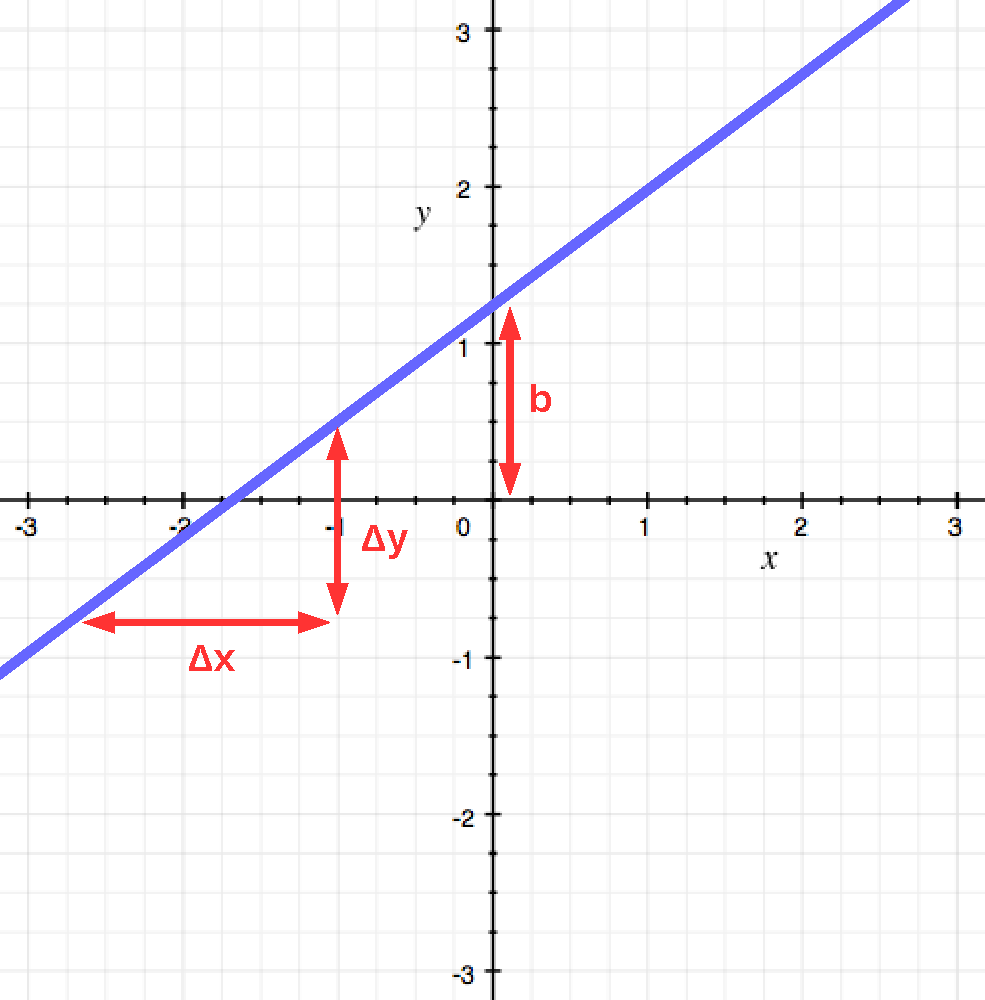
\includegraphics[width=0.9\textwidth]{cart4.pdf}}
  %      \uncover<2>{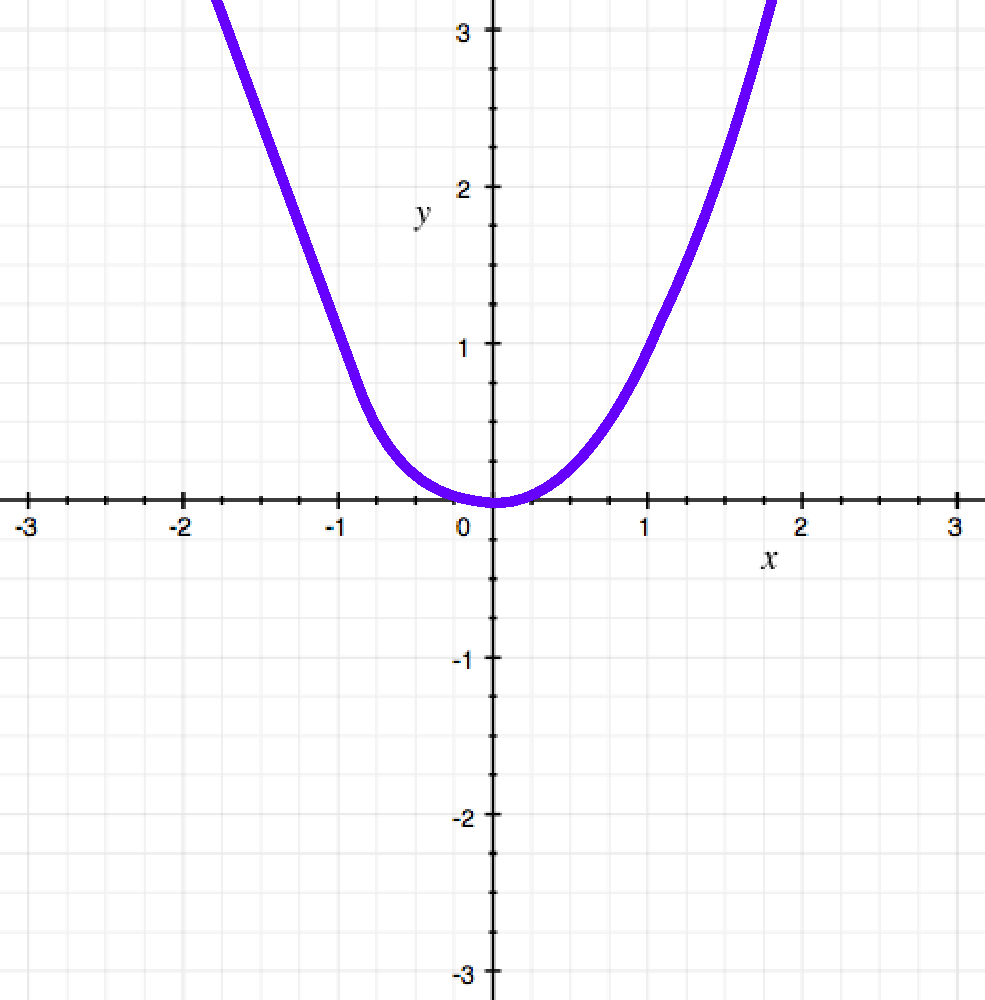
\includegraphics[width=0.9\textwidth]{quad0.pdf}}
  %      \includegraphics<3>[width=0.9\textwidth]{quad1.pdf}
        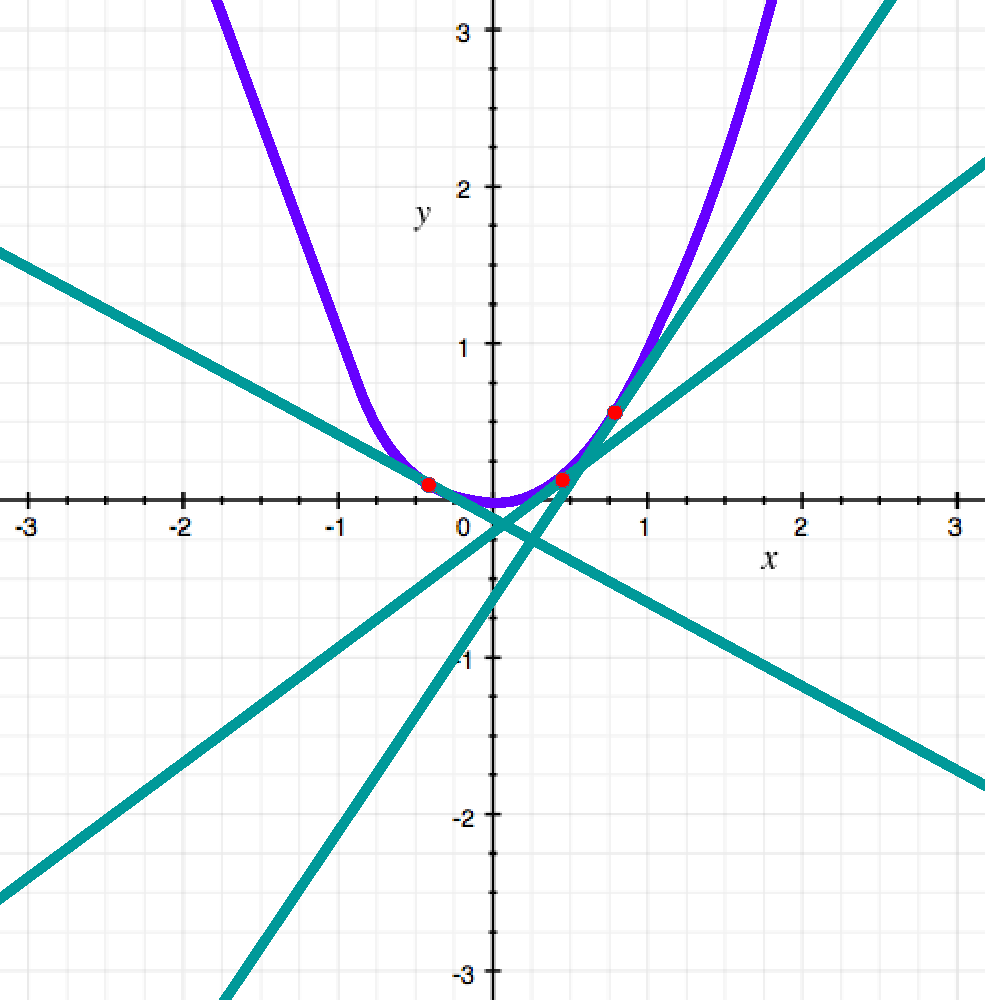
\includegraphics[width=0.9\textwidth]{quad2.pdf}
      \end{center}
    \end{column}
    \begin{column}{0.49\textwidth}
      \begin{itemize}
      \item<1-> We just talked about the slope of a line -- which is a
        constant.
        \begin{itemize}
        \item<2-> But we can also talk about the slope of a curve.
        \item<3-> The slope of a curve is itself a function of the
          variables that define the curve \uncover<4->{$\Rightarrow$ the slope of the series of \alert{tangents}.}
        \end{itemize}
      \item<5-> For a curve defined by $y=x^2$, we can take the
        derivative (aka ``differentiate'', written:
        \begin{block}{}
          \[\frac{dy}{dx} = 2x\]
        \end{block}
      \end{itemize}
    \end{column}
  \end{columns}
}

\pagestepalt{From curves to derivatives}{
  There's a way to ``find'' a derivative that's an extension of the way
  to calculate slope. For function $f(x)$
  \begin{block}{}
    \[\frac{df(x)}{dx} = \lim_{\Delta x \rightarrow 0} \frac{f(x + \Delta x) - f(x)}{\Delta x}\]
  \end{block}\pause
  \begin{itemize}
  \item Taking $m =\frac{\Delta y}{\Delta x}$ as with the linear function
    $y=mx+b$, is just a special,
    simple case of taking $\frac{df(x)}{dx}$. \pause
  \item For a function $F$ over a vector $\mathbf{x}$, we have to take
    ``partial derivatives'' (over each dimension), and we write that as $\nabla F(\mathbf{x}) = (\frac{\partial F}{\partial x_0} \ldots \frac{\partial F}{\partial x_n})$.\pause
  \item (we won't do that in detail\ldots)
  \end{itemize}
}

\placard{Part 3: Exponentiation and logarithms}

\pagestepalt{The rules for logarithms}{
  \vspace{-1cm}
  (Actually they're not rules, they can be proven.)\pause\\
  Consider $N^x$. \pause Then,
  \[\log_N N^x = x\]\pause
  \[N^{\log_N x} = x\]\pause
  \[\log_N a^x = x \log_N a \] \pause
  \[\log_N xy = \log_N x + \log_N y\]\pause
  \[\log_N \frac{x}{y} = \log_N x - \log_N y\]\pause
  And there's more\ldots
}

\pagestepalt{The rules for logarithms}{
  The logarithm of the inverse:
  \[\log_N \frac{1}{x} = -\log_N x\]\pause
  Converting one base into another:
  \[\frac{\log_N x}{\log_N M} = \log_M x\]\pause
  Log of unity:
  \[\log_N 1 = 0\]\pause
  Undefined:
  \[\log_N x = \text{??? if } x \leq 0\]
}

\pagestepalt{Logarithms are useful}{
  Some things we do with logarithms:\pause
  \begin{itemize}
  \item Rescale very large or very small things. (Why?)\pause
  \item Represent choices.\pause
    \begin{itemize}
    \item If there are $N$ choices at any given point in time, and there are are $x$ choices to make, then we have $N^x$ paths into the future.\pause
    \item If we only have the future outcomes, we can ``guess'' how ``complex'' it was to reach those outcomes.\pause
    \item That's why the binary logarithm $\log_2$ is so important.
    \end{itemize}
  \end{itemize}
}

\pagestepalt{$e$}{
  \vspace{-1cm}
  \textbf{Euler's number} $e$ is a very special number in mathematics.
  \begin{block}{}
    \[e \, = 1 + \frac{1}{1} + \frac{1}{1\cdot 2} + \frac{1}{1\cdot 2\cdot 3} + \cdots \, \approx {\bf 2.71828}\]
  \end{block}\pause
  It is used in the exponentiation function $\text{exp}(x) = e^x$ whose inverse
  is the natural logarithm $\ln x$ such that $\ln e^x = x$.\pause\\
  It has a very special property:
  \begin{block}{Differentiating exp}
    \[\frac{de^x}{dx} = e^x\]
  \end{block}
  (ie, it's its own tangent's slope at each point!)
}

\pagestepalt{$e$}{
  \vspace{-1cm}
  Euler's number gets us the very useful (as you'll see)
  \textbf{logistic function}\\\pause
  An S-shaped (`sigmoid') curve, defined as:
  \begin{block}{}
    \[\sigma(x) = \frac{{e}^x}{1 + {e}^x}  = \frac{1}{1 + {e}^{-x}} \]
  \end{block}\pause
  What this looks like:
  \begin{center}
    \raisebox{-2.1em}{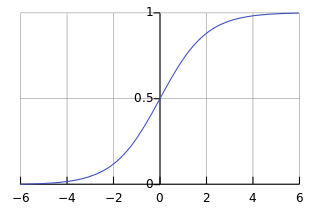
\includegraphics[width=0.27\textwidth]{../images/logistic-curve.png}}
  \end{center}\pause
  This squashes numbers from $(-\infty, \infty)$ to a much smaller
  range $(0, 1)$, with the interesting action happening around the
  middle.
}

\placard{Anything that involves \alert{growth} at a rate proportional to its current size is an $e$-thing!!!}

\placard{Part 4: A little information theory}

\pagestepalt{What does it mean to classify?}{
  In order to classify something (in general) we need to:
  \begin{enumerate}
  \item Determine the possible classes.\pause
  \item Select relevant characteristics that reveal the classes.\pause
  \item Find an empirical basis on which to relate the characteristics
    to the classes. (Including pure speculation?)\pause
  \item Apply those characteristics to a candidate instance.\pause
  \end{enumerate}
  \begin{block}{Classification}
    \textbf{Classification from an ML point of view}: learning a function
    from object characteristics to classes.\\
    $\Rightarrow$ Decision-making.
  \end{block}
}

\pagestepalt{How do we make classification decisions?}{
  (The Na\"{i}ve Bayes approach.)
  \begin{itemize}
  \item Empirical basis:
    \begin{itemize}
    \item Obtain proportions of characteristics (i.e., MLE
      probabilities) in their \alert{contribution} to class
      identification.\pause
    \item Use these characteristics (i.e., \textbf{features}) find the
      most likely class for a given instance given the contribution.
    \end{itemize}
  \end{itemize}\pause
  All features are considered \alert{simultaneously} in the decision
  process and the result is the outcome of a sort of vote.
}

\pagestepalt{But not all features are equal.}{
  Some features are more informative than others. How to quantify this?\pause
  \begin{itemize}
  \item A funny way of looking at it:
    \begin{itemize}
    \item Instances are \alert{encoded messages}.
    \item Classes are the decoded message.
    \end{itemize}\pause
  \item ``Informativeness'' of a feature: how much of the decoded
    message does the feature reveal when its value is observed?
  \end{itemize}
}

\pagestepalt{Encoding messages}{
  A superficial look at (a part of) information theory.\pause
  \begin{itemize}
  \item It is possible to encode a message in \textit{bits}.
    \begin{itemize}
    \item Depending on how many {\it other} messages you expect to receive.
    \item (The notion of a bit is \alert{not necessarily binary}!)
    \end{itemize}\pause
  \item For any ``language'' of encoded messages, there's an average number of bits {\it required} to definitively decode the message.\pause
  \item Let's try it:
    \begin{itemize}
    \item The signal is always ``A''. How many bits required to encode this?\pause
    \item The signal either ``A'' or ``B'', with equal probability. How many bits? \pause
    \item ``A'' or ``B'', but ``A'' is 75\% likely.
    \end{itemize}
  \end{itemize}
}

\pagestepalt{Information in a random variable}{
  \begin{itemize}
  \item Consider a random variable $X$. (Say, coin tosses.) It consists of possible events $x_1 \ldots x_n$.\pause
  \item The probability of any given event in $X$ is given by $P(x_i)$.\pause
  \item The self-information of any event $I(x_i)$ is the number of bits required to encode it, as in $I(x_i)=-\log P(x_i)$. \pause
  \item The \textbf{entropy} $H(X)$ of the entire random variable $X$ is the expected value of its self-information, $I(X)$, or $H(X)=E[I(X)]$\pause
  \end{itemize}
  \begin{block}{Entropy}
    \begin{center}
      $$H(X) = -\sum_{i=1}^{n} P(x_i)I(x_i) = -\sum_{i=1}^{n} P(x_i) \log P(x_i)$$
    \end{center}
  \end{block}
}

\pagestepalt{What can we do with entropy?}{
  The previous definition of entropy tells us how many bits (on average)
  we need to encode the possible outcomes of a \alert{single random event}.\pause
  \begin{itemize}
  \item What if we can break the events into a series?\pause
    \begin{itemize}
    \item Then we can quantify \alert{how much we learned from part of the message}.\pause
    \item Then we can quantify how much we \textbf{might} learn from what we receive next.\pause
    \end{itemize}
  \item This is called the \textbf{information gain} (IG).
  \end{itemize}
  \begin{block}{Information gain}
    \begin{center}
      $$IG(X \vert A) = H(X) - H(X \vert A)$$
    \end{center}
  \end{block}\pause
  (How much you don't know, minus how much you wouldn't know if you knew $A$!)
}

\pagestepalt{Let's take a (little) stab at information gain}{
  Outcomes of two coin flips: HH, HT, TT (treating them as unordered combinations).\pause
  \begin{itemize}
  \item Two events, three ``messages''.\pause
  \item Calculate:
    \begin{itemize}
    \item Entropy with no coin flips. ($H_0$)
    \item Entropy after one coin flip. ($H_1$)
    \item Subtract $H_0 - H_1$ to get information gain.
    \end{itemize}
  \end{itemize}\pause
  We'll do this on the whiteboard (if we have time).
}

%\placard{More dice and Venn diagrams?}

\placard{Part 5: Matrix multiplication}

\pagestepalt{Consider the humble vector}{
  So far, we have written vectors as ordered tuples:
  \[
  \mathbf{x} = (x_1, x_2, \ldots, x_N)
  \]\pause
  It happens that there's another, funny way of writing this:
  \[
  \mathbf{x} = \begin{bmatrix}
    x_1 \\
    x_2 \\
    \vdots \\
    x_N
  \end{bmatrix}\;
  \onslide<3->{\alert{\mathsf{or}}}\;
  \onslide<4->{\mathbf{x} = \begin{bmatrix}
    x_1 & x_2 & \ldots & x_N
  \end{bmatrix}}
  \]
  \onslide<5->{This is \alert{matrix} notation.}
}

\pagestepalt{Dot products in matrix notation}{
  Remember the dot product?
  \[\mathbf{w} \cdot \mathbf{x} = w_1x_1 + w_2x_2 + w_3x_3 + \ldots + w_nx_n\]
  \pause
  In matrix notation, you can write this as:
  \[
  \mathbf{w} \cdot \mathbf{x} =
  \begin{bmatrix}
    w_1 & w_2 & \ldots & w_N
  \end{bmatrix}
  \begin{bmatrix}
    x_1 \\
    x_2 \\
    \vdots \\
    x_N
  \end{bmatrix} =
  \begin{bmatrix}
    w_1x_1 + w_2x_2 + \ldots + w_Nx_N
  \end{bmatrix}
  \]\pause
  That just gives you a 1x1 matrix, so you can drop the brackets. It's \alert{scalar} -- the result of an input vector and a weight vector.
}

\pagestepalt{Multiple weight vectors}{
  Sometimes you need to compute multiple outputs, meaning, you actually
  have multiple \alert{weight vectors} representing multiple equations.\\\pause
  Then you can stack multiple weight vectors into a matrix.
  \[
  \mathbf{W} =
  \begin{bmatrix}
    \mathbf{w_1} \\
    \mathbf{w_2} \\
    \vdots \\
    \mathbf{w_M} 
  \end{bmatrix}
  =
  \begin{bmatrix}
    w_{1,1} & w_{1,2} & \ldots & w_{1,N} \\
    w_{2,1} & w_{2,2} & \ldots & w_{2,N} \\
    \vdots & \vdots & \ldots & \vdots \\
    w_{M,1} & w_{M,2} & \ldots & w_{M,N} 
  \end{bmatrix}
  \]\pause
  This is a matrix with dimensionality MxN.
}

\pagestepalt{Multiple dot products}{
  \vspace{-0.75cm}
  Then we can get multiple outputs of the weight vector.
  \[
  \mathbf{W}\mathbf{x} =
  \begin{bmatrix}
    \mathbf{w_1} \\
    \mathbf{w_2} \\
    \vdots \\
    \mathbf{w_M} 
  \end{bmatrix}
  \begin{bmatrix}
    x_1 \\ x_2 \\ \vdots \\ x_N
  \end{bmatrix}
  =
  \begin{bmatrix}
    w_{1,1} & w_{1,2} & \ldots & w_{1,N} \\
    w_{2,1} & w_{2,2} & \ldots & w_{2,N} \\
    \vdots & \vdots & \ldots & \vdots \\
    w_{M,1} & w_{M,2} & \ldots & w_{M,N} 
  \end{bmatrix}
  \begin{bmatrix}
    x_1 \\ x_2 \\ \ldots \\ x_N
  \end{bmatrix}
  \]\pause\\
  \[
  =
  \begin{bmatrix}
      w_{1,1}x_1 + w_{1,2}x_2 + \ldots + w_{1,N}x_N \\ \vdots \\ w_{M,1}x_1 + w_{M,2}x_2 + \ldots + w_{M,N}x_N 
  \end{bmatrix}
  \]
  \\
  \pause
  Dimensionality MxN and Nx1 result in a vector with dimensionality Mx1, i.e.,
  M outputs for M weight vectors. But the ``inner'' dimensions must match.
}

\pagestepalt{Why do we need this?}{
  \pause Multiple weight vectors.
  \begin{itemize}
  \item Allow us to model more complex interrelationships.\pause
  \item Allow us to produce more outputs from the same data.\pause
  \end{itemize}
  We can also perform mass operations over numerous inputs and weight vectors.
  (This is what GPUs are good at.)\pause
  \[
  \mathbf{W}\mathbf{X} =
  \begin{bmatrix}
    \mathbf{w_1} \\
    \mathbf{w_2} \\
    \vdots\\
    \mathbf{w_M}    
  \end{bmatrix}
  \begin{bmatrix}
    \mathbf{x_1} & \mathbf{x_2} & \ldots & \mathbf{x_L}
  \end{bmatrix}
  =
  \begin{bmatrix}
    \mathbf{W}\mathbf{x_1} & \mathbf{W}\mathbf{x_2} & \ldots & \mathbf{W}\mathbf{x_L}
  \end{bmatrix}
  \]
  \pause and that is \ldots
}

\pagestepalt{Why do we need this?}{
  \ldots a matrix of dimensionality MxL.
  \[
  \mathbf{WX} =
  \begin{bmatrix}
    w_{1,1}x_{1,1} + \ldots + w_{1,N}x_{N,1} & \ldots & w_{1,1}x_{1,L} + \ldots + w_{1,N}x_{N,L} \\ \vdots & \ldots & \vdots \\ w_{M,1}x_{1,1} + \ldots + w_{M,N}x_{N,1} & \ldots & w_{M,1}x_{1,L} + \ldots + w_{M,N}x_{N,L}
  \end{bmatrix}
  \]\pause
  That is, M weights for an N-dimensional vector space, and L inputs
  for of N-dimensions, yields L output vectors for a new, M-dimensional space.
}


\placard{End}

\end{document}
